\documentclass[10pt]{ujarticle}
\usepackage{float}
\usepackage{adrobo_abst}
\usepackage[dvipdfmx]{graphicx}
\usepackage{amssymb,amsmath}
\usepackage{bm}
\usepackage[superscript]{cite}
\usepackage{enumerate}
\usepackage{url}
\usepackage[dvipdfmx]{color}
%\usepackage[absolute]{textpos}

\renewcommand\citeform[1]{(#1)}

\begin{document}
    
    \makeatletter
    \doctype{2022年度卒業論文概要}
    \title{視覚と行動のend-to-end学習により経路追従行動をオンラインで模倣する手法の提案}{(オフラインでデータセットを収集して訓練する手法の提案)}
    \etitle{A proposal for an online imitation method of path-tracking
    behavior by end-to-end learning of vision and action}{(Validation of a method to collect and train dataset offline)}
    
    \author{19C1068\hspace{.5zw}髙橋祐樹}
    \eauthor{Yuuki Takahashi}
    
    \makeatother
    
    \abstract{When preparing the manuscript, read and observe carefully this sample as well as the instruction manual for the manuscript of the Transaction of Japan Society of Mechanical Engineers. This sample was prepared using MS-word. Character size of the English title is 14 pts of Times New Roman as well as sub-title. The name is 12 pts. The address of the first author and the abstract is 10 pts of Times New Roman. Character spacing of the abstract is narrowed by 0.2 pts preferably.}
    
    \keywords{End-to-End Learning, Navigation, Offline}
    
    \maketitle
    
    \supervisor{指導教員:林原靖男 教授}
    
    \section{緒\hspace{2zw}言}%===========================
    近年, 自律移動ロボットの研究が盛んに行われている. その中で視覚を入力としたend-to-end学習により自律走行した例もある. 例えば, Bojarskiら\cite{bojarski}は人が操作するステアリングの角度をend-to-end学習することで, 自律走行する手法を提案した. 本研究室においても, 岡田ら\cite{si2020-okada}\cite{si2021-okada}(以下「従来研究」と称する)により2D-LiDARを用いた自律移動システムの出力をロボットに与えて学習させることで, 経路追従行動をオンラインで模倣する手法を提案し, 実験によりその有効性を確認してきた. 本研究では, 従来手法を基に, 目標とする経路上及び周辺のデータを一度に収集し, オフラインで訓練する手法を提案する. 提案手法では, 経路上にロボットを配置し, カメラ画像と教師データとなる目標角速度を収集する. それらのデータを基にオフラインで学習を行い, 学習後はカメラ画像を入力とした学習出力により自律移動させることで, 手法の有効性を検証する.
    
    \section{従来手法}%===========================
    従来研究の概要を以下で述べる. 従来研究では, 地図を用いたルールベース制御器によるナビゲーションの走行を模倣し, 視覚に基づく経路追従行動を獲得した. 従来研究のシステム概要をに示す. システムでは, LiDAR, オドメトリを入力としたナビゲーションの出力である角速度を学習器とモータ駆動系に与える. ナビゲーションの角速度は, ROSのパッケージであるnavigationにより計算される. また, 学習器には, カメラ画像を64×48にリサイズした3つのカメラ画像を入力し, ナビゲーションの角速度を出力して, 0.2[s]の周期でend-to-end学習する. 左右のカメラ画像に対する目標角速度には, それぞれ経路に戻るようなオフセットを加える. 学習には, に示すような入力層1, 畳み込み層3, 全結合層2, 出力層1の計7層で構成されたネットワークを用いる. 学習後は, カメラ画像のみを入力とした学習器の出力により走行する. 

    % \begin{center}
    %     \begin{figure}[h]
    %         \centering
    %         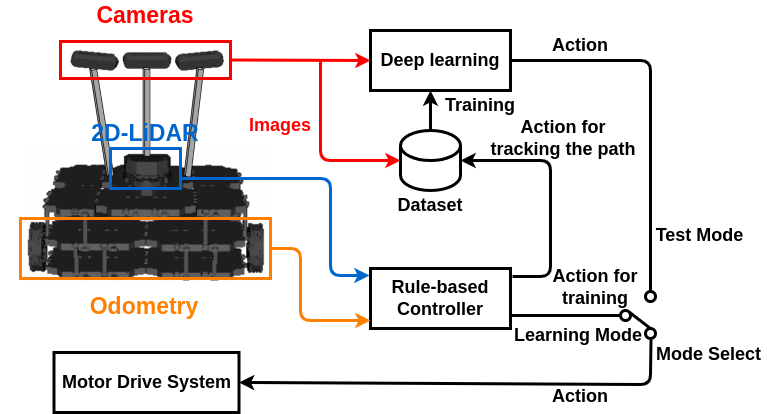
\includegraphics[width=0.45\textwidth]{fig/si2020-okada.png}
    %         \caption{Systems that imitation learning for map-based navigation from \cit{si2020-okada}}
    %         \label{Fig:si2020-okada}
    %     \end{figure}
    % \end{center}

    \section{提案手法}%===========================
    次に, 従来研究を基にしたオフラインでデータを収集し訓練するする手法を提案する. 

    \section{シミュレータを用いた実験}%===========================
    
    \section{結\hspace{2zw}言}%===========================
    
    \vspace{5truemm}
    {\footnotesize
        \begin{thebibliography}{99}

            \bibitem{bojarski}
            Bojarsi, Mariusz, et al.:``End to End Learning for Self-Driving Cars.'', arXiv: 1604.07316, 2016
            
            \bibitem{si2020-okada}
            岡田 眞也, 清岡 優祐, 上田 隆一, 林原 靖男: ``視覚と行動のend-to-end学習により経路追従行動をオンラインで模倣する手法の提案'', \textit{計測自動制御学会 SI 部門講演会 SICE-SI2021 予稿集}, pp.1147-1152, 2020.

            \bibitem{si2021-okada}
            岡田 眞也, 清岡 優祐, 春山 健太, 上田 隆一, 林原 靖男: ``視覚と行動のend-to-end学習により経路追従行動をオンラインで模倣する手法の提案-“経路追従行動の修正のためにデータセットを動的に追加する手法の検討'', \textit{計測自動制御学会 SI 部門講演会 SICE-SI2021 予稿集}, pp.1066-1070, 2021.
            
        \end{thebibliography}
    }
    \normalsize
    
\end{document}
